本节数值均来自P协议；与M同时改变属性、验证图、候选和攻击过程，不能将两轮差值仅归因于EA。
\begin{figure}[H]\centering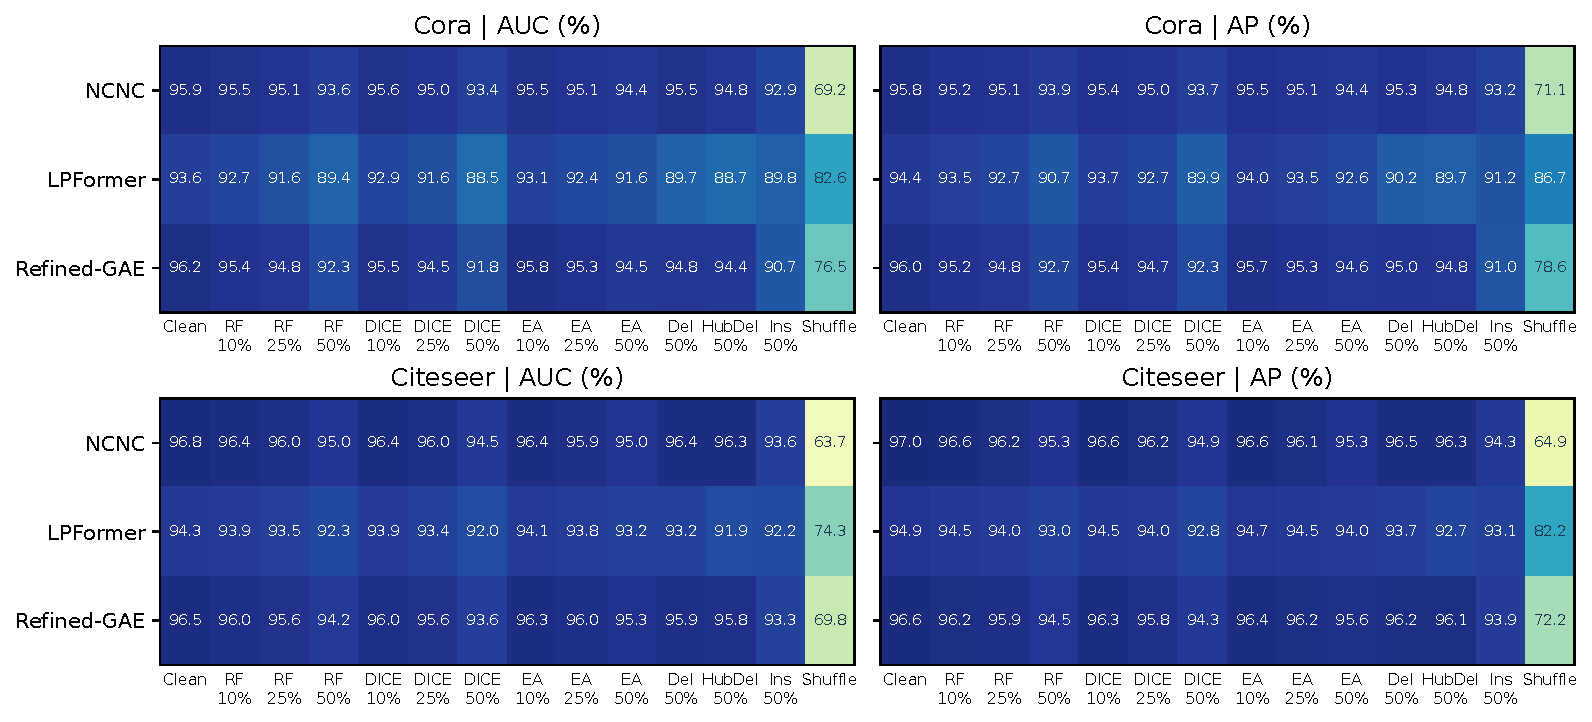
\includegraphics[width=23cm,height=11cm,keepaspectratio]{figures/protected_performance_overview.pdf}\caption{P 协议：完整模型在全部14条件下的 AUC/AP 均值。EA 列的18张实际图均为插边，不代表同时经历删边。}\label{fig:p-overview}\end{figure}
\clearpage
\begin{figure}[H]\centering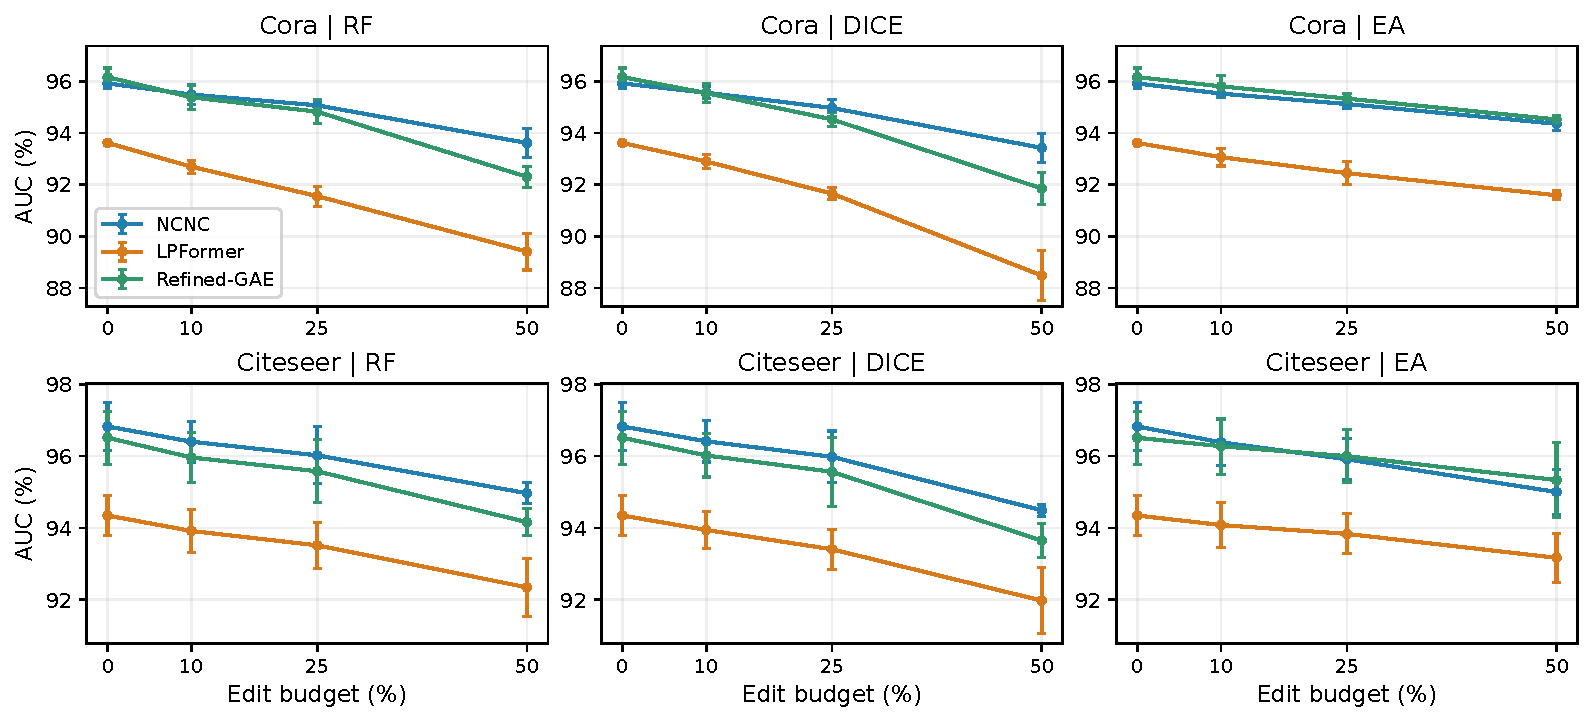
\includegraphics[width=23cm,height=14cm,keepaspectratio]{figures/protected_attack_curves.pdf}\caption{P 协议：RF/DICE/EA 多档预算的 AUC 曲线。此处的预算分母和候选保护规则与 M 不同，不能把两图曲线合并作攻击算法的单变量比较。}\label{fig:p-curves}\end{figure}
\clearpage
\begin{figure}[H]\centering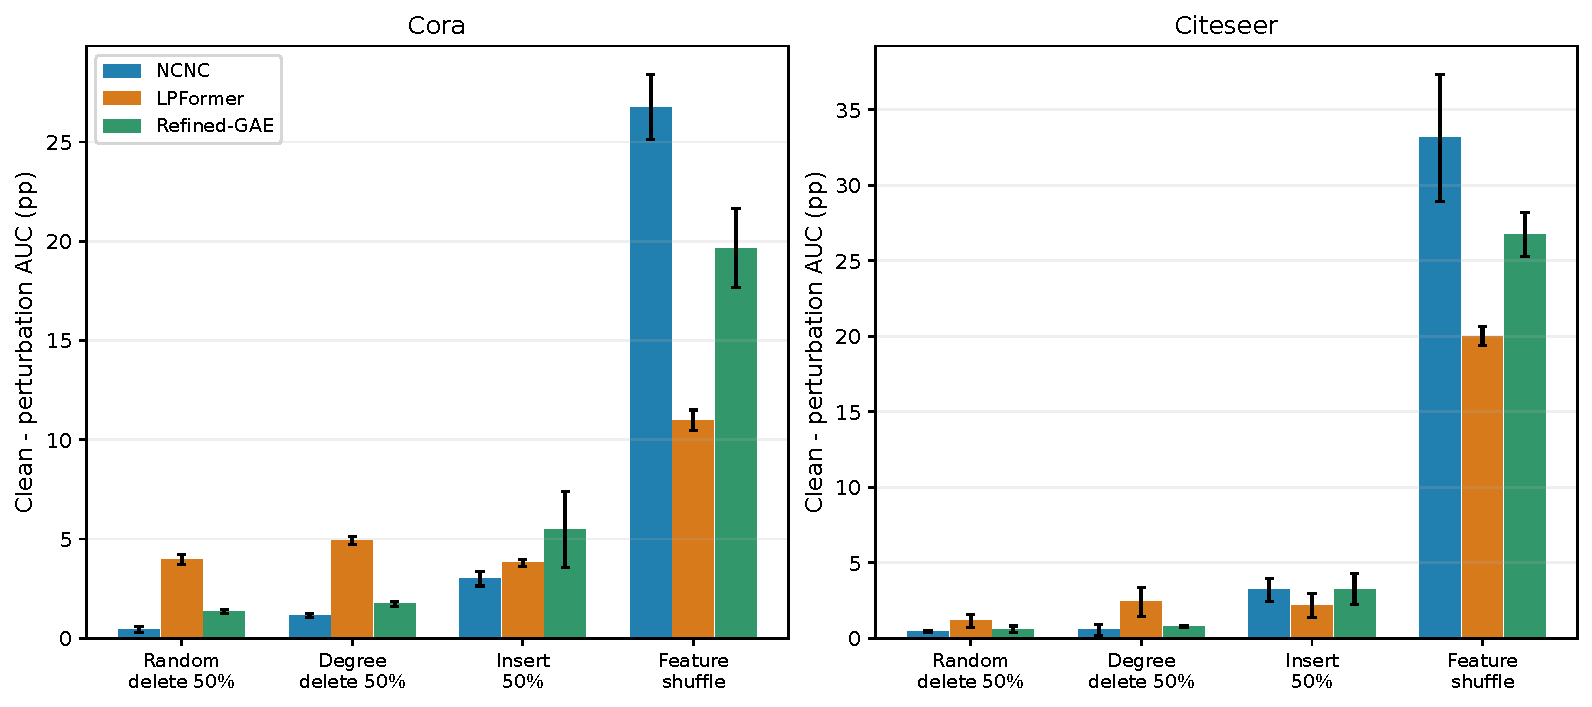
\includegraphics[width=23cm,height=14cm,keepaspectratio]{figures/protected_probe_damage.pdf}\caption{P 协议：纯删边、按度删边、插边和属性置换的配对损失。正降幅表示退化。属性置换检验冻结模型的属性错配敏感性，不是结构-only 重训。}\label{fig:p-probe}\end{figure}
\clearpage
\begin{figure}[H]\centering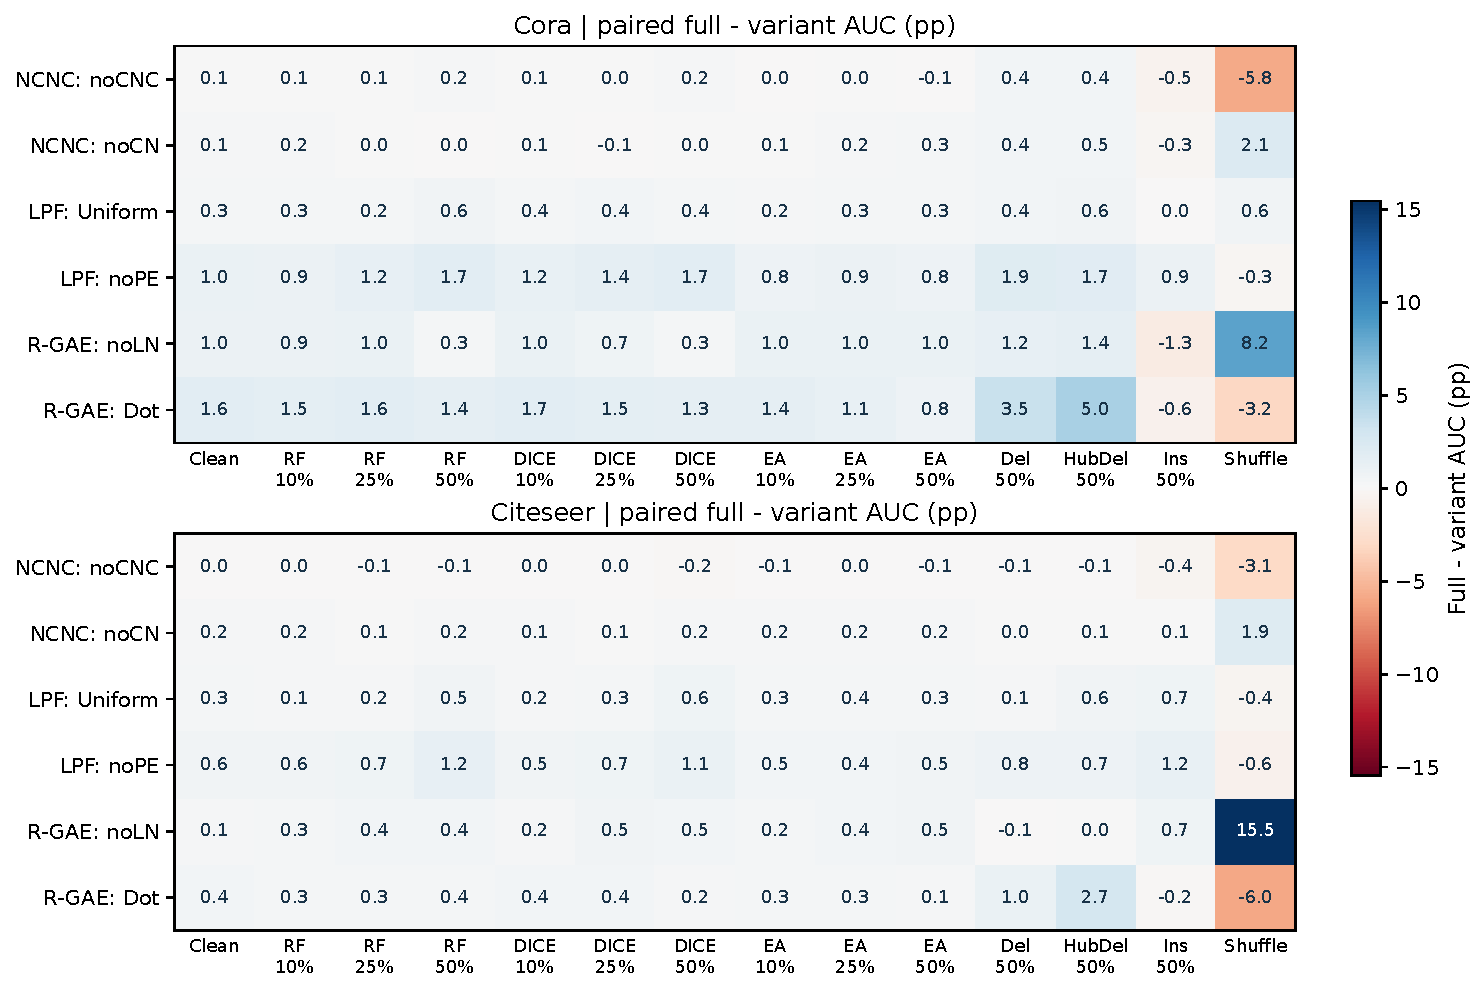
\includegraphics[width=23cm,height=14cm,keepaspectratio]{figures/protected_component_effects.pdf}\caption{P 协议：全部组件的配对效应。与 M 分开报告，检查机制观察是否依赖协议。}\label{fig:p-component}\end{figure}
\end{landscape}
\subsection{纯删边、集中删边与属性错配}
{\footnotesize
\setlength{\tabcolsep}{3.2pt}
\renewcommand{\arraystretch}{1.10}
\begin{longtable}{llrrrrr}
\caption{P 协议完整模型的干净与机制探针 AUC（百分数）}\\
\toprule
数据 & 模型 & Clean & Del50 & HubDel50 & Ins50 & Shuffle \\
\midrule
\endfirsthead
\multicolumn{7}{l}{P 协议完整模型的干净与机制探针 AUC（百分数）（续）}\\
\toprule
数据 & 模型 & Clean & Del50 & HubDel50 & Ins50 & Shuffle \\
\midrule
\endhead
\midrule\multicolumn{7}{r}{续下页}\\
\endfoot
\bottomrule
\endlastfoot
Cora & NCNC & $95.92\pm0.19$ & $95.47\pm0.14$ & $94.77\pm0.31$ & $92.92\pm0.55$ & $69.16\pm1.69$ \\
Cora & LPFormer & $93.61\pm0.08$ & $89.67\pm0.23$ & $88.70\pm0.12$ & $89.82\pm0.25$ & $82.63\pm0.58$ \\
Cora & Refined-GAE & $96.16\pm0.35$ & $94.80\pm0.42$ & $94.43\pm0.25$ & $90.70\pm1.58$ & $76.52\pm1.64$ \\
Citeseer & NCNC & $96.83\pm0.67$ & $96.40\pm0.60$ & $96.27\pm0.77$ & $93.62\pm0.48$ & $63.69\pm3.74$ \\
Citeseer & LPFormer & $94.35\pm0.55$ & $93.20\pm0.71$ & $91.93\pm1.52$ & $92.17\pm0.30$ & $74.34\pm0.39$ \\
Citeseer & Refined-GAE & $96.51\pm0.73$ & $95.90\pm0.60$ & $95.75\pm0.80$ & $93.27\pm0.67$ & $69.80\pm0.72$ \\
\end{longtable}
}

NCNC 在随机纯删边50\%下，Cora/Citeseer 的 AUC 分别为 $95.47\pm0.14$、$96.40\pm0.60$；按度加权删边后为 $94.77\pm0.31$、$96.27\pm0.77$。LPFormer 对应随机删边为 $89.67\pm0.23$、$93.20\pm0.71$，按度删边为 $88.70\pm0.12$、$91.93\pm1.52$；Refined-GAE 分别为 $94.80\pm0.42$、$95.90\pm0.60$ 以及 $94.43\pm0.25$、$95.75\pm0.80$。这组证据来自真正的纯删边探针，与旧EA的插边性质分开解释。

属性置换下 NCNC 的 Cora/Citeseer AUC 为 $69.16\pm1.69$、$63.69\pm3.74$，LPFormer 为 $82.63\pm0.58$、$74.34\pm0.39$，Refined-GAE 为 $76.52\pm1.64$、$69.80\pm0.72$。NCNC 的结构编辑表现较稳，却不代表对属性与节点错配稳健。不同扰动轴不能合并为一个没有条件限制的“robustness好”。

\subsection{组件、注意力与传播行为}
P 协议中，完整 NCNC 减 noCNC 的干净配对 AUC 为 Cora $0.06\pm0.27$、Citeseer $-0.01\pm0.26$，同样没有支持较大的普遍补全收益。Cora LPFormer 减 noPE 为 $0.98\pm1.10$，减 Uniform 为 $0.32\pm0.59$；与 M 的 PubMed 观察方向并不一致，说明需要限定数据与协议。

每种子取前64正例和64负例分析完整 LPFormer，共每数据集384个点对。候选数不超过1的比例为 Cora69.27\%、Citeseer77.60\%，平均候选数2.20/1.06；这类点对没有多候选权重分配的空间。在候选数大于1的抽样点对中，平均归一化熵约0.071/0.166。Uniform 的归一化熵在多候选时为1，noPE 的编码输出为零；这是实现核验与行为描述，注意力集中不等于因果解释。

Refined-GAE 在 P 中，完整减 Dot 的 Cora 干净 AUC 为 $1.57\pm0.50$，DICE50 为 $1.34\pm0.13$。属性置换时，完整减 noLN 为 Cora $8.22\pm6.68$、Citeseer $15.46\pm1.99$；它显示归一化组与属性错配表现有关，但编码器/解码器 LayerNorm 尚未分别消融。完整模型四个传播深度的平均 softmax 系数为 Cora约$(0.260,0.349,0.208,0.183)$、Citeseer约$(0.291,0.281,0.214,0.214)$，只描述混合行为，不能读成各深度的因果贡献比例。

干净图分层表在附录展开，正负类内的分数相关、全扰动分层与抽样注意力原始数据随源码提交。分层避免混淆不同共同邻居/度/属性相似度的候选，但小样本层会不稳定，AP也受正例占比变化影响。这些统计是解释线索，不替代控制变量消融。
